%% This is file `elsarticle-template-1a-num.tex',
%%
%% Copyright 2009 Elsevier Ltd
%%
%% This file is part of the 'elsarticle Bundle'.
%% ---------------------------------------------
%%
%% It may be distributed under the conditions of the LaTeX Project Public
%% License, either version 1.2 of this license or (at your option) any
%% later version.  The latest version of this license is in
%%    http://www.latex-project.org/lppl.txt
%% and version 1.2 or later is part of all distributions of LaTeX
	%% version 1999/12/01 or later.
%%
%% The list of all files belonging to the 'Elsarticle Bundle' is
%% given in the file `manifest.txt'.
%%
%% Template article for Elsevier's document class `elsarticle'
%% with numbered style bibliographic references
%%
%% $Id: elsarticle-template-1a-num.tex 151 2009-10-08 05:18:25Z rishi $
%% $URL: http://lenova.river-valley.com/svn/elsbst/trunk/elsarticle-template-1a-num.tex $
%%
%\documentclass[preprint,12pt]{elsarticle}

%% Use the option review to obtain double line spacing
%% \documentclass[preprint,review,12pt]{elsarticle}

%% Use the options 1p,twocolumn; 3p; 3p,twocolumn; 5p; or 5p,twocolumn
%% for a journal layout:
%% \documentclass[preprint]{elsarticle}
%% \documentclass[final,1p,times,twocolumn]{elsarticle}
 \documentclass[preprint,3p,times]{elsarticle}
%% \documentclass[final,3p,times,twocolumn]{elsarticle}
%% \documentclass[final,5p,times]{elsarticle}
%% \documentclass[final,5p,times,twocolumn]{elsarticle}

%% if you use PostScript figures in your article
%% use the graphics package for simple commands
%% \usepackage{graphics}
%% or use the graphicx package for more complicated commands
%% \usepackage{graphicx}
%% or use the epsfig package if you prefer to use the old commands
%% \usepackage{epsfig}

%% The amssymb package provides various useful mathematical symbols
\usepackage{amssymb}
\usepackage{subfigure}
\usepackage{graphicx}
\usepackage{listings}
\usepackage{url}
\usepackage{booktabs,colortbl,array,color,tabularx,subfigure}
\usepackage[T1]{fontenc}
\usepackage{amsmath}
\usepackage[brazilian]{babel}
\usepackage[utf8]{inputenc}

\newcommand{\foops}[1]{\mbox{\texttt{#1}}}
\newcommand{\code}[1]{\foops{#1}}
%% The amsthm package provides extended theorem environments
%% \usepackage{amsthm}

%% The lineno packages adds line numbers. Start line numbering with
%% \begin{linenumbers}, end it with \end{linenumbers}. Or switch it on
%% for the whole article with \linenumbers after \end{frontmatter}.
%% \usepackage{lineno}

%% natbib.sty is loaded by default. However, natbib options can be
%% provided with \biboptions{...} command. Following options are
%% valid:

%%   round  -  round parentheses are used (default)
%%   square -  square brackets are used   [option]
%%   curly  -  curly braces are used      {option}
%%   angle  -  angle brackets are used    <option>
%%   semicolon  -  multiple citations separated by semi-colon
%%   colon  - same as semicolon, an earlier confusion
%%   comma  -  separated by comma
%%   numbers-  selects numerical citations
%%   super  -  numerical citations as superscripts
%%   sort   -  sorts multiple citations according to order in ref. list
%%   sort&compress   -  like sort, but also compresses numerical citations
%%   compress - compresses without sorting
%%
%% \biboptions{comma,round}

% \biboptions{}


% \journal{Information and Software Technology}

\begin{document}
\begin{frontmatter}

%% Title, authors and addresses

%% use the tnoteref command within \title for footnotes;
%% use the tnotetext command for the associated footnote;
%% use the fnref command within \author or \address for footnotes;
%% use the fntext command for the associated footnote;
%% use the corref command within \author for corresponding author footnotes;
%% use the cortext command for the associated footnote;
%% use the ead command for the email address,
%% and the form \ead[url] for the home page:
%%
%% \title{Title\tnoteref{label1}}
%% \tnotetext[label1]{}
%% \author{Name\corref{cor1}\fnref{label2}}
%% \ead{email address}
%% \ead[url]{home page}
%% \fntext[label2]{}
%% \cortext[cor1]{}
%% \address{Address\fnref{label3}}
%% \fntext[label3]{}

\title{Projeto de Estat\'istica - 2013.1}

%% use optional labels to link authors explicitly to addresses:
%% \author[label1,label2]{<author name>}
%% \address[label1]{<address>}
%% \address[label2]{<address>}

\author{Paola Rodrigues, Rodrigo Andrade}
\address{Centro de Inform\'atica
\\ Universidade Federal de Pernambuco
\\prga,rcaa2@cin.ufpe.br
}

\begin{abstract}
Este documento refere-se...
\end{abstract}

\end{frontmatter}

%%
%% Start line numbering here if you want
%%
% \linenumbers

%% main text

\section{Justificativa}

\label{sec:justificativa}

%De início, explicitam-se os motivos que justificam a pesquisa, determinando-se e delimitando-se o problema, 
%o qual deve estar formulado de maneira clara e precisa

Engenharia de Linhas de Produto de Software (LPS) é uma abordagem de
desenvolvimento que reusa de forma estratégica uma base comum de artefatos que
implementam um conjunto de sistema similares que compartilham características em
comum, mas também são suficientemente distintos entre si. Alguns dos benefícios
esperados por essa abordagem são: redução de \emph{time-to-market} para
lançamento de novos produtos, redução do esforço de manutenção e,
indiretamente, a melhora da qualidade dos produtos~\cite{pohl-book}.

Nesse contexto, a atividade de testes de LPS tem sido considerada um desafio,
principalmente devido a enorme quantidade de produtos gerados por uma LPS e
também porque os requisitos variam de um produto para o outro de forma que não
existe uma especificação única que contemple todos os possíveis fluxos dos
produtos de uma linha. Para lidar com esses problemas, várias técnicas que
derivam casos de testes funcionais para produtos específicos dentro de uma LPS
tem sido propostas como PLUTO~\cite{Bertolino:pluto} e
ScenTED~\cite{Pohl:scented}. No entanto, apesar de várias propostas de solução, 
essa área de pesquisa ainda não possui uma quantidade satisfatória de avaliações
empíricas que tragam análises e evidências sobre o benefício na prática de se
utilizar casos de teste específicos por produto

Essa falta de discussões pode ser um dos fatores que acabe por desencorajar a
indústria a adotar tais técnicas~\cite{Tevanlinna:spltesting, Engstrom2011}.
Como resultado, pelo que observamos em um ambiente de execução de testes na
indústria, empresas comumente descrevem o comportamento dos produtos de uma
mesma linha de uma maneira genérica, descrevendo os passos mais comuns entre os
produtos e abstraindo o fato de que alguns passos são opcionais ou alternativos
e algumas vezes até omitindo tais passos. Por exemplo, um caso de teste que
especifica um cenário de uma funcionalidade de geração de relatórios pode conter
todos os possíveis formatos de arquivos de relatório como PDF, HTML, XLS, e
testadores utilizariam esse teste para testar todos os produtos da linha, mesmo
no caso em que os produtos gerados não possuam todas essas opções de formato de
relatórios. 

No entanto, as abstrações contidas nas suítes genéricas podem comprometer a
execução manual dos testes, pois os testadores, que devem seguir estritamente o
passo-a-passo descrito nos testes, podem se confundir. Essa confusão pode levar
a consequências indesejadas tais como defeitos escapados -- aqueles defeitos que
só são descobertos após o lançamento do produto no mercado -- e defeitos que são
reportados mas não existem -- o que afeta a produtividade do processo de
execução dos testes.

Alternativamente, com a adoção de uma técnica de especificação de testes para
uma LPS,

 Nesse trabalho
apresentamos estudos que comparam empiricamente duas técnicas de desenvolvimento de casos de teste. Uma técnica genérica observada em um ambiente
real de execução de testes e uma técnica de casos de teste específicos por
produto cujos testes poderiam ser obtidos através de qualquer uma das técnicas
de derivação de testes existente. Para comparar essas técnicas, conduzimos 5
experimentos controlados avaliando o impacto das técnicas sob o ponto de vista
do processo de execução de testes, coletando métricas relacionadas ao esforço
de execução de testes. Após a análise dos dados coletados alcançamos resultados
que sugerem benefícios, tais como redução do tempo de execução, que
a indústria poderia alcançar ao adotar uma técnica de derivação de testes.





\section{Fundamenta\c{c}\~ao te\'orica}

\label{sec:fundamentacao}

\section{Objetivo da pesquisa}
\label{sec:objetivos}
%Os objetivos devem ser retirados diretamente dos problemas levantados no Passo 2. 
%Define-se o que se pretende alcançar com a realização do trabalho.
Nesse trabalho, temos como objetivo executar uma avaliação empírica que compara
duas técnicas de \emph{design} de testes para LPS, a TG e a TE. Esse estudo visa
comparar e analisar essas técnicas sob o ponto de vista do processo de execução
dos testes quanto a sua eficiência, medida por meio do tempo necessário para
executar suítes de teste em cada uma. Com esse estudo, temos a finalidade de
investigar os benefícios e desvantagens que essas técnicas possuem na prática,
trazendo assim, alguma evidência para aqueles que desejem optar por uma ou por
outra.


\section{Especifica\c{c}\~ao da amostra}
\label{sec:especificacao}

% Deve-se determinar a área de execução da pesquisa, a população a ser investigada, o tipo de amostra e a determinação do seu tamanho, bem como o tipo de amostragem a ser utilizado. Define-se as variáveis envolvidas.

Nesta seção, nós determinamos a área de execução da pesquisa, a população investigada, o tamanho da amostra e as variáveis envolvidas.

A área de execução da pesquisa é inserida no contexto de estratégias de testes para Linhas de Produto de Software (LPS)~\cite{pohl-book}. Para atingir os objetivos mencionados na Seção~\ref{sec:objetivos}, um experimento foi definido para investigar como uma população lidaria com as duas estratégias de testes para LPS e consequentemente, trazendo evidências de qual estratégia é a melhor.

Esse experimento foi definido usando a abordagem Goal (objetivo), Question (pergunta) e Metric (métrica) (GQM)~\cite{gqm}. Primeiramente, definimos o objetivo, que é analisar o processo de execução de teste das duas estratégias considerando a eficiência em termos de tempo de execução. Segundo, definimos a pergunta de pesquisa: A TE reduz o esforço de execução do teste comparado com a TG? Por último, definimos uma métrica: tempo de execução dos testes.

Para realizar esse experimento definido, utilizamos uma população composta por 18 alunos de pós-graduação. Eles foram divididos em duplas e usaram as estratégias TE e TG para testar um conjunto de features em uma LPS. Durante esse experimento, coletamos o tempo de execução da suites de testes de cada dupla, cada estudante de uma dada dupla, associados a feature e técnica que usaram para formar nossa amostra. A Tabela~\ref{tab:amostra} exibe uma parte pequena dessa amostra que coletamos e analisamos\footnote{Os dados completos podem ser obtidos em: https://github.com/rcaa/ProjetoEstatistica2013/tree/master/dados}, como detalhado na Seção~\ref{sec:analise}. As variáveis envolvidas são número da dupla, estudante, feature, técnica e tempo de execução.

\begin{table}[h]\footnotesize
    \caption{Dados da amostra}
    \centering
    \begin{tabular}{|l|l|l|l|l|}
    \addlinespace
    \hline
    {\bf Nº da dupla}  & {\bf Estudante} & {\bf Feature} & {\bf Técnica} & {\bf Tempo de execução}\\ \hline
    1 & 1 & F1 & TG & 880\\ \hline
    1 & 1 & F2 & TE & 841\\ \hline
    \end{tabular}
  \label{tab:amostra}
\end{table}

Nós determinamos um número de 18 pessoas para constituir a população com o intuito de simular como seria um ambiente de testes em uma organização de tamanho médio. Dessa forma, nossa amostra considera 36 entradas, ou seja, 36 linhas diferentes na tabela acima. Ela leva em conta as combinações possíveis entre nossas variáveis.



\section{An\'alise da amostra}
\label{sec:analise}
%Fazer um estudo descritivo dos dados (gráficos e medidas). Verificar normalidade dos dados e potenciais pontos aberrantes

Nesta seção, nós apresentamos um estudo descritivo dos dados da amostra. Nesse contexto, mostramos alguns gráficos gerados por meio da linguagem R, bem como verificamos a normalidade dos dados.

\subsection{Estudo descritivo}
\label{sec:estudo}

%falar sobre os gráficos e medidas que vamos usar




\subsection{Normalidade dos dados}
\label{sec:normalidade}

Para demonstrar a normalidade dos resíduos dos dados da nossa amostra, nós usamos o teste de aderência Shapiro-Wilk~\cite{shapirowilk}. Ele testa a hipótese nula de que uma amostra foi proveniente de uma população com distribuição normal. Portanto, se o \emph{p-value} for menor do que o nível de significância escolhido, então a hipótese nula é rejeitada, ou seja, os dados não foram provenientes de uma população com distribuição normal. Por outro lado, se o \emph{p-value} for maior que o nível de significância, então a hipótese nula não é rejeitada e consequentemente, os dados são provenientes de uma população com distribuição normal. A seguir, nós formalizamos a hipótese desse teste:

\begin{equation}
	H_{0} : \text{A amostra provém de uma população Normal}
\end{equation}

\begin{equation}
	H_{1} : \text{A amostra não provém de uma população Normal}
\end{equation}

Nesse contexto, aplicando o teste Shapiro-Wilk, nós obtivemos um \emph{p-value} igual a 0,1456, que é maior que o nosso nível de significância 0,05. Portanto, 1 não pode ser rejeitada, o que traz evidências de que os resíduos dos dados da nossa amostra provém de uma população com distribuição normal. Além disso, esse teste é baseado na estatística W~\cite{estatisticaw}. Nós obtemos um W igual a 0,9546, o que é maior que o valor 0,935 dado na tabela com os valores críticos da estatística W. Desse modo, o nosso W sendo maior que o W fornecido pela tabela\footnote{Tabela pode ser obtida em: https://github.com/rcaa/ProjetoEstatistica2013/blob/master/images/shapiro-wilk.pdf}, temos fortes evidências de normalidade dos resíduos dos dados da nossa amostra.

Esse teste de aderência pode ser interpretado por um gráfico Quantile-Quantile Plot ou Q-Q Plot. Esse gráfico ilustra se os resíduos dos dados de uma amostra provêm de uma população com distribuição normal. Além disso, ele exibe os \emph{quantiles} da amostra contra os \emph{quantiles} teóricos~\cite{Wilk1968}. Com isso, é possível visualizar a aderência dos resíduos dos dados à Normal. Na Figura~\ref{fig:grafico1}, nós ilustramos a nossa análise. A reta que cruza o gráfico representa a Normal. Percebe-se que os nossos dados estão muito próximos dessa reta, com exceção somente de 4 dos 36 pontos. Portanto, o gráfico Q-Q Plot também confirma que nossa amostra é Normal.

\begin{figure*}[t]
	\caption{Q-Q Plot}
    \centering
    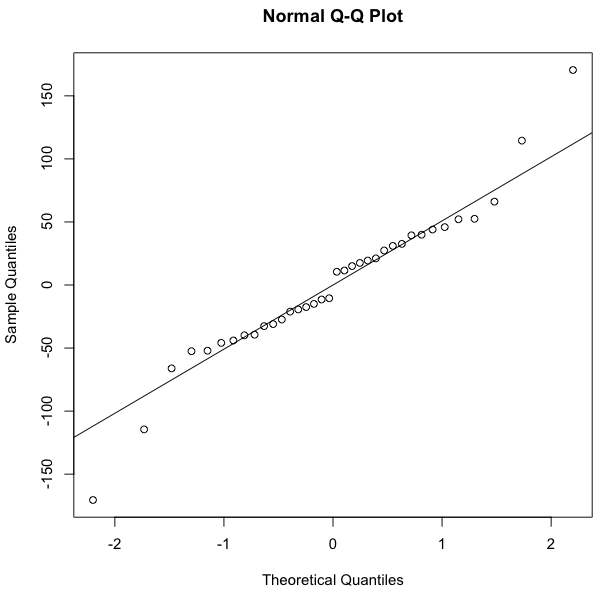
\includegraphics[width=0.4\textwidth]{images/qqplot.png}
    \caption{}
    \label{fig:grafico1}
\end{figure*}

\section{Metodologia}
\label{sec:metodologia}

%Estabelecem-se as hipóteses a serem formuladas, as quais devem ser claras e precisa. 


%Ta faltando isso aqui:
%Define-se o problema estatisticamente, decidindo-se que informação estatística é realmente necessária e qual método que será aplicado.

Nesta seção, estabelecemos as hipóteses e definimos o problema estatisticamente.

Primeiramente, definimos as hipóteses para a primeira questão de pesquisa (Seção~\ref{sec:especificacao}), ou seja, queremos saber se a ST reduz o esforço de execução do teste comparado com a GT:

\begin{equation}
	H_{0} : \mu_{TempoST} \geq \mu_{TempoGT}
\end{equation}

\begin{equation}
	H_{1} : \mu_{TempoST} < \mu_{TempoGT}
\end{equation}

Em que (1) é a hipótese nula e (2) é a hipótese alternativa. Portanto, a equação 1 representa a hipótese de o tempo consumido para executar as suites de teste com a estratégia ST é maior ou igual ao consumido usando GT, enquanto que (2) representa a hipótese de o tempo consumido com a estratégia ST é menor que com a GT.

Já considerando a segunda questão de pesquisa, ou seja, se o uso de ST reduz o número de CRs terminadas em comparação com GT, nós definimos as seguintes hipóteses:

\begin{equation}
	H_{0} : \mu_{CRsTerminadasST} \geq \mu_{CRsTerminadasGT}
\end{equation}

\begin{equation}
	H_{1} : \mu_{CRsTerminadasST} < \mu_{CRsTerminadasGT}
\end{equation}

Em que (1) é a hipótese nula e (2) é a hipótese alternativa. Portanto, a equação 1 representa a hipótese de o número de CRs terminadas usando ST seja maior ou igual ao resultado usando GT, enquanto que a equação 2 representa a situação inversa, ou seja, o número de CRs terminadas com ST é menor que com GT.





\section{An\'alise dos resultados}
\label{sec:resultados}

% Passa-se ao tratamento dos dados por intermédio dos testes estatísticos, os quais dependem das hipóteses a serem testadas. Nesse tópico, é exigido que sejam aplicados testes de hipóteses paramétricos e/ou não paramétricos. Testes de duas amostras são exigidos quando comparando abordagens

Nessa seção, nós mostramos como tratamos os resíduos dos dados da amostra por intermédio dos testes estatísticos. 

Para interpretar os dados, nós primeiramente conduzimos uma análise descritiva para observar tendência nos dados baseada em algumas características como dispersão e mediana. Nós elaboramos o gráfico Boxplot ilustrado na Figura~\ref{fig:boxplot} para comparar a execução das estratégicas TE e TG. Esse gráfico mostra que o tempo de execução dos testes tende a ser menor para TE. A média para completar as atividades usando TG foi de 975 segundos, enquanto que a média para TG foi de 824 segundos. A TE teve uma diminuição média de 15\% no tempo de execução. No mais, nenhuma discrepância apareceu no gráfico.

\begin{figure}[t]
    \centering
    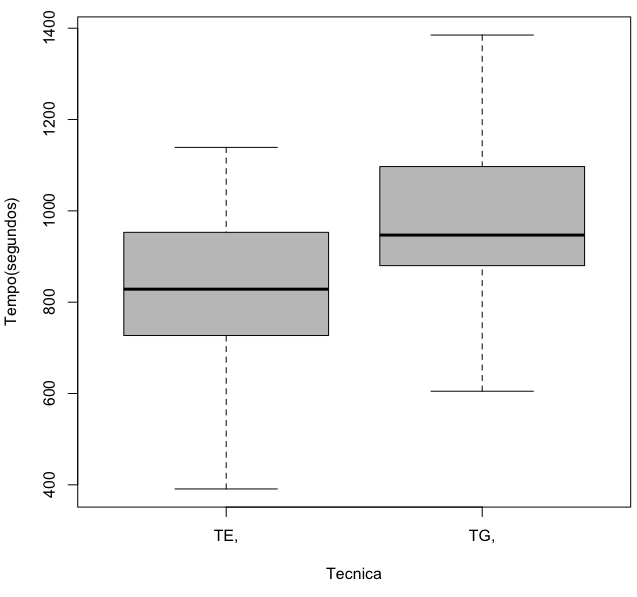
\includegraphics[width=0.4\textwidth]{images/boxplot.png}
    \caption{}
    \label{fig:boxplot}
\end{figure}

% mostrar o dotplot também aqui
Além do Boxplot, nós também elaboramos o gráfico Dotplot ilustrado na Figura~\ref{fig:dotplot} para termos uma visão diferente da análise. Com esse gráfico, podemos ver para cada um dos 18 estudantes, representados de A a R, que o uso da técnica TE (Específico) para executar os testes levou menos tempo do que que TG (Genérico). A única exceção foi o estudante P. Outro ponto importante, é que a feature (F1 ou F2) usada não influencia nos resultados.

\begin{figure}[t]
    \centering
    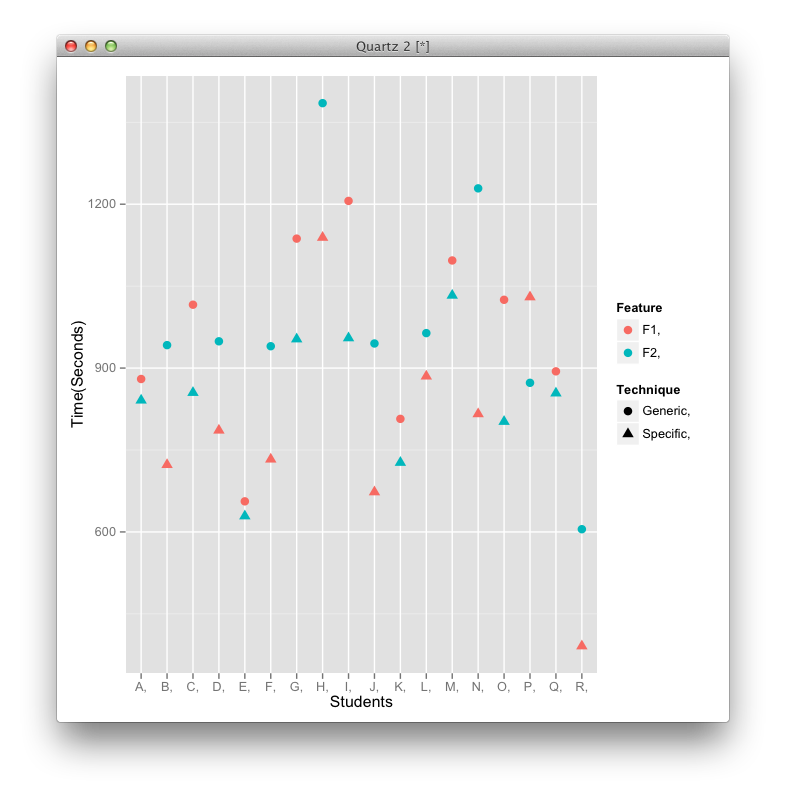
\includegraphics[width=0.4\textwidth]{images/dotplot.png}
    \caption{}
    \label{fig:dotplot}
\end{figure}

Além dos valores da mediana, nós queríamos comparar as observações de acordo com cada resultado das estratégias (TE e TG). Nós pudemos observar para ambas as estratégias que não importa a feature usada para executar os casos de testes, 94\% dos estudantes terminaram em menos tempo usando TE. Dos 18 alunos analisados, só um levou mais tempo para executar os testes com TE.

Continuando com a análise estatística, nós queremos verificar se a tendência observada nas nossas amostras foi de fato significante. Para verificar isso, nós rodamos teste de hipótese paramétrico baseado na média. Nesse contexto, nós usamos o ANOVA como dito na Seção~\ref{sec:metodologia}. Nós executamos o teste ANOVA e alcançamos um \emph{p-value} para o fator da estratégia de aproximadamente 0,0001, o que nos dá evidência significante de que a estratégia TE pode reduzir o tempo de execução das suites de testes.

Todo código escrito em R, dados e fontes do texto podem ser acessados livremente no nosso repositório: \\https://github.com/rcaa/ProjetoEstatistica2013

%% The Appendices part is started with the command \appendix;
%% appendix sections are then done as normal sections
%% \appendix

%% \section{}
%% \label{}

%% References
%%
%% Following citation commands can be used in the body text:
%% Usage of \cite is as follows:
%%   \cite{key}          ==>>  [#]
%%   \cite[chap. 2]{key} ==>>  [#, chap. 2]
%%   \citet{key}         ==>>  Author [#]

%% References with bibTeX database:

%\bibliographystyle{elsarticle-num}
\bibliographystyle{elsarticle-num}
\bibliography{RCAA}

%% Authors are advised to submit their bibtex database files. They are
%% requested to list a bibtex style file in the manuscript if they do
%% not want to use model1a-num-names.bst.

%% References without bibTeX database:

% \begin{thebibliography}{00}

%% \bibitem must have the following form:
%%   \bibitem{key}...
%%

% \bibitem{}

% \end{thebibliography}


\end{document}

%%
%% End of file `elsarticle-template-1a-num.tex'.
